\chapter{Software Architecture \& Finite State Machine}

\section{System Architecture Overview}
The software architecture runs on FreeRTOS on the ESP32-S3 and keeps sensor collection, decision-making, and motor control separate. Although the ESP32-S3 has two cores, explicit core pinning was not needed; FreeRTOS SMP is used to spread the sensor tasks across the available cores. This keeps the path-planning code responsive and less affected by polling delays.

Data flows in one direction: Sensors $\rightarrow$ FSM $\rightarrow$ Navigation (APF) $\rightarrow$ Motor Control. 

\begin{figure}[h]
    \centering
    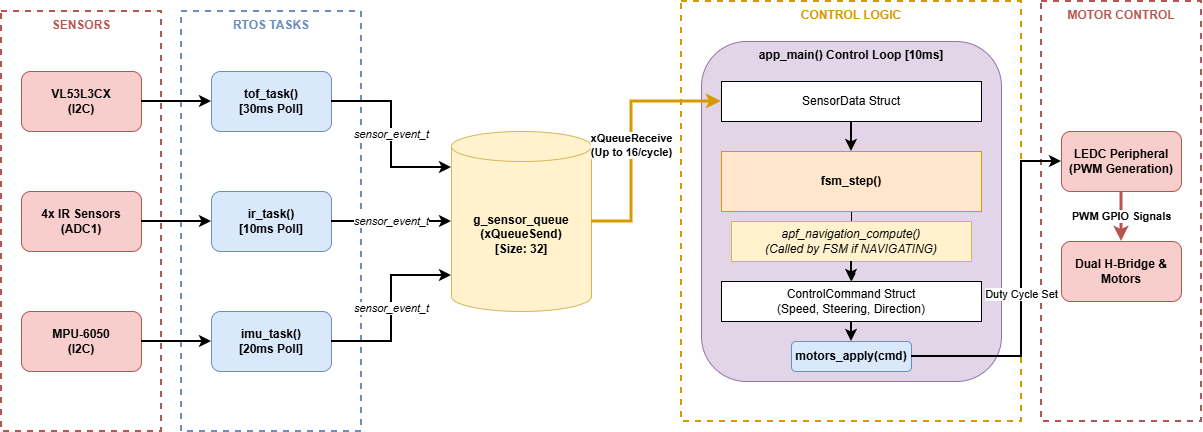
\includegraphics[width=1.2\textwidth]{images/SoftwareArchitecture.drawio.png}
    \caption{Overall software architecture showing the queue-based sensor pipeline, FSM, navigation, and motor control layers}
    \label{fig:software_architecture}
\end{figure}

\FloatBarrier

\section{Hardware Abstraction Interfaces}
Data structures sit between the subsystems so the higher-level logic does not need to read hardware registers or work directly with raw PWM output.

\subsection{SensorData Struct}
The \texttt{SensorData} structure normalises all inputs before they reach the navigation logic. Infrared (IR) readings are calibrated onto a scale from 0.0 for white floor to 1.0 for black tape, and the Time-of-Flight (ToF) reading is converted into centimetres. This keeps the path-planning algorithm independent of the sensor hardware and mounting height.

\subsection{ControlCommand Struct}
Motor commands are standardised through a \texttt{ControlCommand} structure with three fields:
\begin{itemize}
    \item \textbf{Speed:} A normalised float between \texttt{0.0} and \texttt{1.0}.
    \item \textbf{Steering:} A normalised float between \texttt{-1.0} (full left) and \texttt{1.0} (full right).
    \item \textbf{Direction:} An integer representing forward (\texttt{+1}) or reverse (\texttt{-1}).
\end{itemize}
Keeping navigation separate from raw PWM output makes the APF module independent of the L298N H-bridge, so hardware changes or motor retuning do not affect the algorithm.
\section{RTOS Task Management \& The 100Hz Control Loop}
The ToF, IR, and IMU sensors each run in their own FreeRTOS task. Rather than overwriting global variables, which risks race conditions, each task packages its reading into a \texttt{sensor\_event\_t} packet and sends it to the thread-safe FreeRTOS queue (\texttt{g\_sensor\_queue}).

To stop fast-polling sensors from starving the FSM or tripping the watchdog, the central control task handles at most 16 events per cycle. It then uses \texttt{vTaskDelayUntil()} to maintain a 100Hz, or 10ms, control loop. That steady timing helps with smooth trajectory calculations and accurate IMU integration.

\section{IMU Processing \& Dynamic Bias Calibration}
MEMS gyroscopes such as the MPU-6050 suffer from zero-bias drift and can report non-zero angular velocity even when the vehicle is still. If that error is left uncorrected, heading drift builds up over time.

The system updates the gyroscope bias whenever the vehicle is at rest. It treats the vehicle as stationary when the gyroscope magnitude stays below $12^{\circ}/s$ and the accelerometer reads roughly Earth's gravity ($1g \pm 0.2g$) for at least 0.5 seconds. During these periods, the zero-bias is updated with an Exponential Moving Average (EMA) filter:

$$ \alpha = \frac{\Delta t}{\tau + \Delta t} $$
$$ bias_{new} = (1 - \alpha) \cdot bias_{old} + \alpha \cdot \omega_{raw} $$

Where $\Delta t$ is the polling interval and $\tau$ is the time constant. Once the vehicle starts moving, the bias update stops. The stored bias is then subtracted from the raw yaw rate ($\omega_{raw}$) before the value reaches the FSM. 

\section{Finite State Machine (FSM)}
The system is governed by a Finite State Machine configured through a central \texttt{SystemConfig} struct, which keeps the runtime thresholds and delays in one place.

\begin{figure}[h]
    \centering
    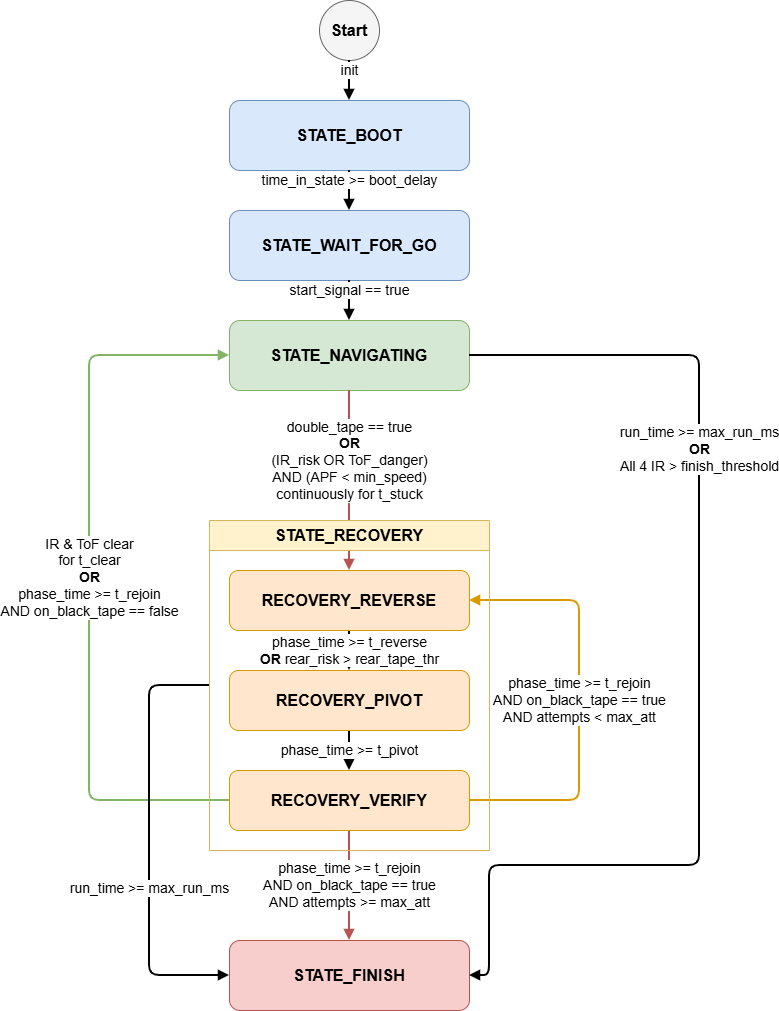
\includegraphics[width=1.2\textwidth]{images/fsm.drawio.png}
    \caption{Finite state machine for boot, wait, navigation, recovery, and finish handling}
    \label{fig:fsm}
\end{figure}

\FloatBarrier

\begin{itemize}
    \item \textbf{STATE\_BOOT:} A required 750ms delay immediately after power-on. This gives the ToF and IR sensors time to initialise before the system starts reading data.
    \item \textbf{STATE\_WAIT\_FOR\_GO:} The system idles until the user presses the ESP32 BOOT button to start the run.
    \item \textbf{STATE\_NAVIGATING:} The main operating state. Sensor data is fed into the Artificial Potential Field (APF) to produce the \texttt{ControlCommand}. The FSM also watches for the finish line, which is detected when all four IR sensors exceed the black-tape threshold at the same time.
    \item \textbf{STATE\_RECOVERY:} An autonomous intervention state triggered when the vehicle becomes stuck.
    \item \textbf{STATE\_FINISH:} Reached either by crossing the finish line or by exceeding the 2-minute run limit. All motor outputs are set to zero.
\end{itemize}

\section{APF Local Minima Detection \& Recovery Routing}
A known limitation of Artificial Potential Fields is the local minima problem. For example, if the vehicle drives into a 90-degree corner, the repulsive forces from the black tape can cancel out and the APF may command zero target speed. The vehicle then becomes stuck. Strictly proportional APF implementations can also produce a ping-pong effect when the vehicle bounces between corridor walls because the control loop has no damping.

To reduce high-frequency lateral oscillations, the APF target heading ($\theta_{raw}$) is damped using the real-time yaw rate ($\omega_{yaw}$) from the IMU. An adjustable damping gain ($K_{damping}$) converts angular velocity into a steering penalty and smooths out large command spikes during rapid rotation:

$$ \theta_{target} = \theta_{raw} - (\omega_{yaw} \cdot K_{damping}) $$

To avoid getting stuck in local minima, the FSM checks whether the vehicle is in a high-risk zone, based on ToF and IR proximity, while the APF speed command stays below the minimum threshold (\texttt{min\_apf\_speed}, set to 0.03). If that condition lasts for the timeout period (\texttt{t\_stuck\_ms} = 500ms), the FSM transitions to \textbf{STATE\_RECOVERY}. A double-tape panic override is also used: if both front IR sensors report high risk at the same time, the FSM skips the timeout and enters recovery immediately to keep the vehicle inside the field boundary.

The recovery sequence operates in three sub-phases:
\begin{enumerate}
    \item \textbf{REVERSE:} The vehicle briefly stops to lose forward momentum, then reverses. A steering bias is applied based on which front IR sensor sees the highest risk, which helps pivot the rear wheels into free space. Reversing stops immediately if the rear IR sensors detect tape.
    \item \textbf{PIVOT:} The vehicle shifts into forward gear and steers sharply away from the danger zone to break the APF's local minima equilibrium.
    \item \textbf{VERIFY:} The vehicle resumes APF control under a strict speed limit. It must see clear floor, using safe IR and ToF readings, for a continuous period of \texttt{t\_clear\_ms} before returning to \textbf{STATE\_NAVIGATING}. If tape is detected during verification, the recovery cycle repeats.
\end{enumerate}